% \section{IMU误差模型}

% \begin{comment}
% \end{comment}
% \begin{frame}
% \frametitle{确定性误差标定 \hfill 
\includegraphics[height=0.5cm]{00_logo.png}}
% \begin{columns}
%   \column{0.1\textwidth}
  
%   \column{0.8\textwidth}
%   IMU不依托额外设备实现标定

%   \begin{itemize}
%     \item aa
% %  \item 参考论文:[A Robust and Easy to Implement Method for IMU Calibration without External Equipments ](http://www.dis.uniroma1.it/~pretto/papers/tpm_icra2014.pdf)
  
%  \item DEMO链接:https://bitbucket.org/alberto_pretto/imu_tk
%   \end{itemize}


  
%   % \column{0.3\textwidth}
% 	% \begin{figure}[h]
% 	% 	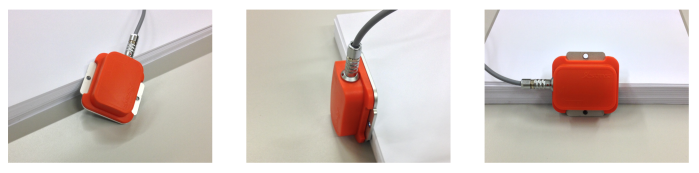
\includegraphics[trim=1.5 0 0 0, height=3.5cm,clip]{13_1.png}
% 	% 	% \caption{四个区域搜索空间}
%   % \end{figure}
  
% 	\column{0.1\textwidth}

% \end{columns}
% \end{frame}

%%%%%%%%%%%%%%%%%%%%%%%%%%%%

\begin{comment}
\end{comment}
\begin{frame}
\frametitle{IMU确定性误差标定(不依托额外设备法) \hfill 
\includegraphics[height=0.5cm]{00_logo.png}}
\begin{columns}
  \column{0.1\textwidth}
  
  \column{0.8\textwidth}
  
  \begin{itemize}
    % \item 参考论文:[A Robust and Easy to Implement Method for IMU Calibration without External Equipments ](http://www.dis.uniroma1.it/~pretto/papers/tpm_icra2014.pdf)
    \item 参考论文:\href{http://www.dis.uniroma1.it/~pretto/papers/tpm_icra2014.pdf}{A Robust and Easy to Implement Method for IMU Calibration without External Equipments} 
    \item DEMO链接:https://bitbucket.org/alberto\_pretto/imu\_tk
  \end{itemize}
  % \column{0.3\textwidth}
	\begin{figure}[h]
		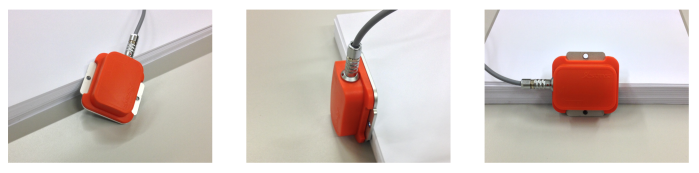
\includegraphics[trim=1.5 0 0 0, height=3.5cm,clip]{13_1.png}
		% \caption{四个区域搜索空间}
  \end{figure}
  
	\column{0.1\textwidth}

\end{columns}
\end{frame} 



%%%%%%%%%%%%%%%%%%%%%%%%%%%%

\begin{comment}
\end{comment}
\begin{frame}
\frametitle{IMU确定性误差标定(不依托额外设备法) \hfill 
\includegraphics[height=0.5cm]{00_logo.png}}
\begin{columns}
  \column{0.1\textwidth}
  
  \column{0.6\textwidth}
  
  IMU数据录制步骤:
  \begin{enumerate}
    \item Left the IMU static for 50 seconds.
    \item Rotate the IMU and then lay it in a different attitude.
    \item Wait for at least 1 seconds.
    \item Have you rotated the IMU 36 - 50 times? If not, go back to step 2.
    \item Done.
  \end{enumerate}
  
  \column{0.2\textwidth}
	\begin{figure}[h]
		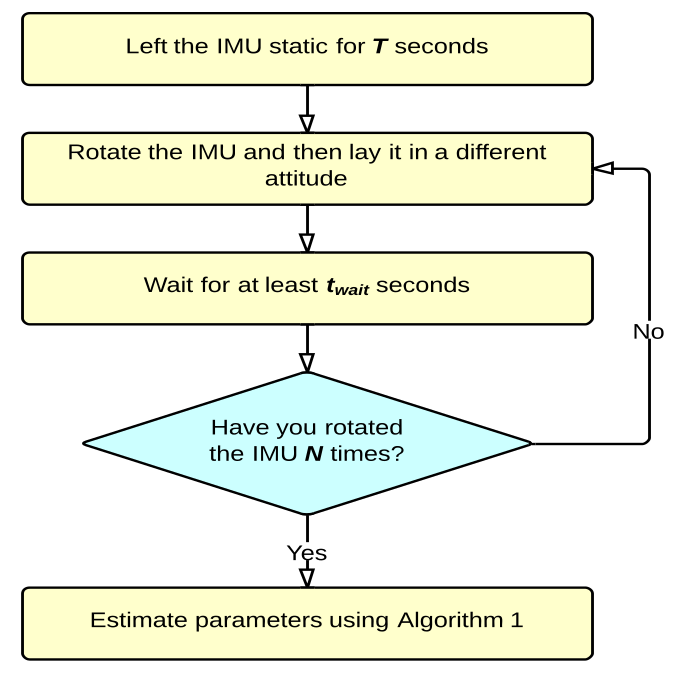
\includegraphics[trim=1.5 0 0 0, height=3.5cm,clip]{13_2.png}
		% \caption{四个区域搜索空间}
  \end{figure}
  
	\column{0.1\textwidth}

\end{columns}
\end{frame} 

%%%%%%%%%%%%%%%%%%%%%%%%%%%%

\begin{comment}
\end{comment}
\begin{frame}
\frametitle{IMU确定性误差标定(不依托额外设备法) \hfill 
\includegraphics[height=0.5cm]{00_logo.png}}
\begin{columns}
  \column{0.1\textwidth}
  
  \column{0.4\textwidth}
  % 确定性误差模型:
  % \begin{equation*}
  %   \begin{split}
  %     \begin{bmatrix}
  %       l_{ax} \\ l_{ay} \\ l_{az}
  %     \end{bmatrix} = 
  %     \begin{bmatrix}
  %       b_{ax} \\ b_{ay} \\ b_{az}
  %     \end{bmatrix} +
  %     \begin{bmatrix}
  %       s_{xx} & m_{xy} & m_{xz} \\
  %       m_{yx} & s_{yy} & m_{yz} \\
  %       m_{zx} & m_{zy} & s_{zz}
  %     \end{bmatrix} \cdot 
  %     \begin{bmatrix}
  %       a_x \\ a_y \\ a_z
  %     \end{bmatrix}
  %   \end{split}
  % \end{equation*}

  (IG1)加速度计确定性误差标定结果:
  \begin{figure}[h]
		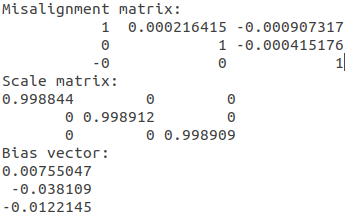
\includegraphics[trim=1.5 0 0 0, height=3.5cm,clip]{13_3.png}
		% \caption{四个区域搜索空间}
  \end{figure}
  
  % IMU确定性误差校正步骤:
  % \begin{enumerate}
  %   \item Left the IMU static for 50 seconds.
  %   \item Rotate the IMU and then lay it in a different attitude.
  %   \item Wait for at least 1 seconds.
  %   \item Have you rotated the IMU 36 ~ 50 times? If not, go back to step 2.
  %   \item Done.
  % \end{enumerate}
  
  \column{0.4\textwidth}
  (IG1)陀螺仪确定性误差标定结果:
	\begin{figure}[h]
		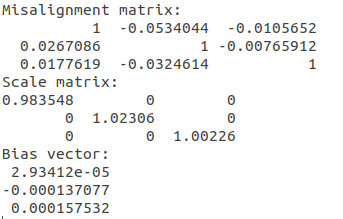
\includegraphics[trim=1.5 0 0 0, height=3.5cm,clip]{13_4.png}
		% \caption{四个区域搜索空间}
  \end{figure}
  
	\column{0.1\textwidth}

\end{columns}
\end{frame} 


